\documentclass[11pt,respuestas,a4]{aleph-examen}
% \documentclass[11pt,a4]{aleph-examen}

% -- Paquetes extra
\usepackage{aleph-comandos}
\usepackage{systeme}
\usepackage{tikz}
\usetikzlibrary{calc,babel}

% -- Datos
\institucion{Facultad de Ciencias Exactas, Naturales y Ambientales}
\carrera{Catálogo STEM}
\asignatura{Matemática III}
\tema{Repaso -- Criterio 2.3}
\autor{Andrés Merino}
\fecha{Periodo 2026-1}

\logouno[0.16\textwidth]{Logos/logoPUCE_04_ac}
\definecolor{colortext}{HTML}{1957d1}
\definecolor{colordef}{HTML}{1957d1}
\fuente{montserrat}


\begin{document}

\encabezado


\begin{preguntas}

%%%%%%%%%%%%%%%%%%%%%%%%%%%%%%%%%%%%%%%%%%
\item
Calcule la integral doble
\[
    \iint_R \left(xy^2 + 2x\right)\,dA,
    \qquad
    R = [0,2]\times[1,3].
\]

\begin{respuesta}
Como $R$ es un rectángulo, por el Teorema de Fubini podemos plantear la integral doble como una integral iterada:
\[
    \iint_R \left(xy^2 + 2x\right)\,dA
    =
    \int_0^2 \left(\int_1^3 \left(xy^2 + 2x\right)\,dy\right) dx.
\]
Integremos primero la integral interna, respecto de $y$:
\[
    \int_1^3 \left(xy^2 + 2x\right)\,dy
    =
    \left.\left(\frac{xy^3}{3} + 2xy\right)\right|_1^3
    =
    \left(9x + 6x\right) - \left(\frac{x}{3} + 2x\right)
    =
    \frac{38}{3}x.
\]
Con esto, integramos respecto de $x$:
\[
    \iint_R \left(xy^2 + 2x\right)\,dA
    =
    \int_0^2 \frac{38}{3}x\,dx
    =
    \left.\frac{38}{3}\cdot\frac{x^2}{2}\right|_0^2
    =
    \frac{38}{3}\cdot 2
    =
    \frac{76}{3}.\qedhere
\]
\end{respuesta}


%%%%%%%%%%%%%%%%%%%%%%%%%%%%%%%%%%%%%%%%%%
\item
Calcule la integral doble
\[
    \iint_D 6xy\,dA,
\]
donde $D$ es la región acotada por las curvas $y = x^2$ e $y = x$.

\begin{respuesta}
Primero, determinemos la región de integración. Las curvas $y=x^2$ e $y=x$ se cortan cuando
\[
    x^2 = x
    \quad\Longleftrightarrow\quad
    x(x-1) = 0
    \quad\Longleftrightarrow\quad
    x = 0 \ \text{ o }\ x = 1.
\]
Para $x\in[0,1]$ se tiene que $x^2 \le x$, por lo que la región puede describirse como una región de Tipo I:
\[
    D = \left\{(x,y) : 0\le x\le 1,\ x^2 \le y \le x\right\}.
\]
\begin{center}
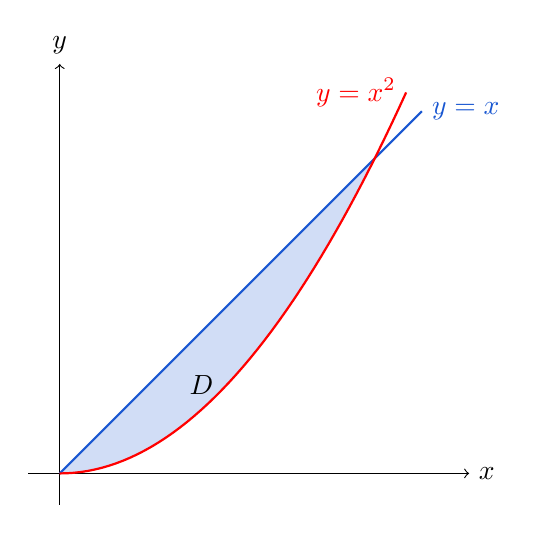
\begin{tikzpicture}[scale=4]
    \draw[->] (-0.1,0) -- (1.3,0) node[right] {$x$};
    \draw[->] (0,-0.1) -- (0,1.3) node[above] {$y$};
    \fill[colordef!20]
        plot[domain=0:1, samples=50] (\x,{\x}) --
        plot[domain=1:0, samples=50] (\x,{\x*\x}) -- cycle;
    \draw[colordef, thick, domain=0:1.15, samples=50] plot (\x,{\x}) node[right] {$y=x$};
    \draw[red, thick, domain=0:1.1, samples=50] plot (\x,{\x*\x}) node[left] {$y=x^2$};
    \node at (0.45,0.28) {$D$};
\end{tikzpicture}
\end{center}
Con esto, planteamos la integral doble como una integral iterada:
\[
    \iint_D 6xy\,dA
    =
    \int_0^1 \left(\int_{x^2}^{x} 6xy\,dy\right) dx.
\]
Integremos primero la integral interna, respecto de $y$:
\[
    \int_{x^2}^{x} 6xy\,dy
    =
    \left.\left(3xy^2\right)\right|_{x^2}^{x}
    =
    3x\cdot x^2 - 3x\cdot x^4
    =
    3x^3 - 3x^5.
\]
Finalmente, integramos respecto de $x$:
\[
    \int_0^1 \left(3x^3 - 3x^5\right)\,dx
    =
    \left.\left(\frac{3x^4}{4} - \frac{3x^6}{6}\right)\right|_0^1
    =
    \frac{3}{4} - \frac{1}{2}
    =
    \frac{1}{4}.\qedhere
\]
\end{respuesta}


%%%%%%%%%%%%%%%%%%%%%%%%%%%%%%%%%%%%%%%%%%
\item
Considere la integral doble
\[
    \iint_D x^2\,dA,
\]
donde $D$ es la región del primer cuadrante acotada por las hipérbolas $xy = 1$, $xy = 3$ y las rectas $y = x$, $y = 4x$. Mediante el cambio de variable
\[
    u = xy,\qquad v = \frac{y}{x},
\]
{plantee} la integral como una integral iterada en las variables $u$ y $v$ (no es necesario evaluarla).

\begin{respuesta}
Con el cambio de variable $u = xy$, $v = y/x$, despejemos $x$ y $y$ en términos de $u$ y $v$: multiplicando ambas expresiones, $x^2 = u/v$; dividiéndolas, $y^2 = uv$. Como estamos en el primer cuadrante, tomamos las raíces positivas, de modo que la transformación $T$ y su inversa están dadas por
\[
    T(u,v) = (x,y) = \left(\sqrt{\frac{u}{v}},\ \sqrt{uv}\right).
\]
Las curvas que acotan a $D$ se transforman en:
\[
    xy = 1 \ \Rightarrow\ u = 1,
    \qquad
    xy = 3 \ \Rightarrow\ u = 3,
    \qquad
    y = x \ \Rightarrow\ v = 1,
    \qquad
    y = 4x \ \Rightarrow\ v = 4.
\]
Por lo tanto, la región en las nuevas variables es el rectángulo
\[
    D' = \left\{(u,v) : 1\le u\le 3,\ 1\le v\le 4\right\}.
\]
Calculemos el jacobiano de la transformación $T$:
\[
    \det\bigl(J_T(u,v)\bigr)
    =
    \det\begin{pmatrix}
        \dfrac{\partial x}{\partial u} & \dfrac{\partial x}{\partial v}\\[10pt]
        \dfrac{\partial y}{\partial u} & \dfrac{\partial y}{\partial v}
    \end{pmatrix}
    =
    \det\begin{pmatrix}
        \dfrac{1}{2\sqrt{uv}} & -\dfrac{1}{2v}\sqrt{\dfrac{u}{v}}\\[10pt]
        \dfrac{1}{2}\sqrt{\dfrac{v}{u}} & \dfrac{1}{2}\sqrt{\dfrac{u}{v}}
    \end{pmatrix}
    =
    \frac{1}{4v} + \frac{1}{4v}
    =
    \frac{1}{2v}.
\]
Además, como $x^2 = u/v$, el integrando se transforma en $x^2 = \dfrac{u}{v}$. Con esto, la integral planteada como integral iterada es
\[
    \iint_D x^2\,dA
    =
    \int_1^4 \int_1^3 \frac{u}{v}\left|\det\bigl(J_T(u,v)\bigr)\right|\,du\,dv
    =
    \int_1^4 \int_1^3 \frac{u}{v}\cdot\frac{1}{2v}\,du\,dv
    =
    \int_1^4 \int_1^3 \frac{u}{2v^2}\,du\,dv.\qedhere
\]
\end{respuesta}


%%%%%%%%%%%%%%%%%%%%%%%%%%%%%%%%%%%%%%%%%%
\item
Sea el sólido
\[
    R = \left\{(x,y,z) : 1\le x\le 2,\ 0\le y\le x^2,\ 0\le z\le x+y\right\}.
\]
{Plantee} la integral triple
\[
    \iiint_R xy\,dV
\]
como una integral iterada (indicando claramente los límites de integración).

\begin{respuesta}
La descripción del sólido $R$ proporciona directamente los límites de integración: $x$ varía entre las constantes $1$ y $2$; para cada $x$, la variable $y$ varía entre $0$ y $x^2$; y para cada $(x,y)$, la variable $z$ varía entre $0$ y $x+y$. Integrando en el orden $dz\,dy\,dx$, la integral iterada es
\[
    \iiint_R xy\,dV
    =
    \int_1^2 \int_0^{x^2} \int_0^{x+y} xy\,dz\,dy\,dx.\qedhere
\]
\end{respuesta}


%%%%%%%%%%%%%%%%%%%%%%%%%%%%%%%%%%%%%%%%%%
\item
Sea el campo escalar $f(x,y) = 2x + \sqrt{y}$ y la trayectoria
\[
    \alpha(t) = (t,\ t^2),\qquad 0\le t\le 1.
\]
{Plantee} la integral de línea
\[
    \int_C f\,ds
\]
como una integral definida respecto del parámetro $t$ (no es necesario evaluarla).

\begin{respuesta}
Recordemos que, para una trayectoria $\alpha(t)$ con $t\in[a,b]$, la integral de línea de un campo escalar es
\[
    \int_C f\,ds = \int_a^b f\bigl(\alpha(t)\bigr)\,\norma{\alpha'(t)}\,dt.
\]
Calculemos cada elemento. La derivada de la trayectoria y su norma son
\[
    \alpha'(t) = (1,\ 2t),
    \qquad
    \norma{\alpha'(t)} = \sqrt{1 + 4t^2}.
\]
Evaluando el campo escalar sobre la trayectoria (con $t\ge 0$, de modo que $\sqrt{t^2}=t$):
\[
    f\bigl(\alpha(t)\bigr) = 2t + \sqrt{t^2} = 2t + t = 3t.
\]
Con esto, la integral de línea planteada como integral definida es
\[
    \int_C f\,ds = \int_0^1 3t\,\sqrt{1 + 4t^2}\,dt.\qedhere
\]
\end{respuesta}


%%%%%%%%%%%%%%%%%%%%%%%%%%%%%%%%%%%%%%%%%%
\item
Sea el campo vectorial $\mathbf{F}(x,y) = (x^2,\ xy)$ y la misma trayectoria del ejercicio anterior,
\[
    \alpha(t) = (t,\ t^2),\qquad 0\le t\le 1.
\]
{Plantee} la integral de línea
\[
    \int_C \mathbf{F}\cdot d\mathbf{r}
\]
como una integral definida respecto del parámetro $t$ (no es necesario evaluarla).

\begin{respuesta}
Recordemos que, para una trayectoria $\alpha(t)$ con $t\in[a,b]$, la integral de línea de un campo vectorial es
\[
    \int_C \mathbf{F}\cdot d\mathbf{r} = \int_a^b \mathbf{F}\bigl(\alpha(t)\bigr)\cdot \alpha'(t)\,dt.
\]
Calculemos cada elemento. La derivada de la trayectoria es $\alpha'(t) = (1,\ 2t)$, y el campo vectorial evaluado sobre la trayectoria es
\[
    \mathbf{F}\bigl(\alpha(t)\bigr) = \bigl(t^2,\ t\cdot t^2\bigr) = (t^2,\ t^3).
\]
El producto escalar del integrando es
\[
    \mathbf{F}\bigl(\alpha(t)\bigr)\cdot \alpha'(t) = (t^2)(1) + (t^3)(2t) = t^2 + 2t^4.
\]
Con esto, la integral de línea planteada como integral definida es
\[
    \int_C \mathbf{F}\cdot d\mathbf{r} = \int_0^1 \bigl(t^2 + 2t^4\bigr)\,dt.\qedhere
\]
\end{respuesta}

\end{preguntas}

\end{document}
